\documentclass[a4j, twocolumn]{jarticle}
% \documentclass[a4j]{jarticle}

\usepackage[dvipdfmx]{graphicx}
\usepackage{subcaption}
\usepackage{caption}

\begin{document}
\title{Queen}
\author{イマム カイリ ルビス\thanks{情報工学分野}}
\date{\today}

\maketitle

\section{クイーンについて}
クイーンは,1970年にロンドンでり結成されたイギリスのロックバンドである.初期の作品はプログレッシブロック,ハードロック,ヘヴィメタルの影響を受けていたが,次第にアリーナロックやポップロックなどのスタイルを取り入れ,よりコンベンショナルな作品へと変化していった.\\
クイーンのメンバー:
\begin{itemize}
  \item フレディマーキュリー(リードボーカル,ピアノ)
  \item ブライアンメイ(ギター,ボーカル)
  \item ロジャーテイラー(ドラム,ボーカル)
  \item ジョンディーコン(ベース)
\end{itemize}

\begin{figure}[htb]
  \centering
  \begin{subfigure}[b]{0.15\textwidth}
      \centering
      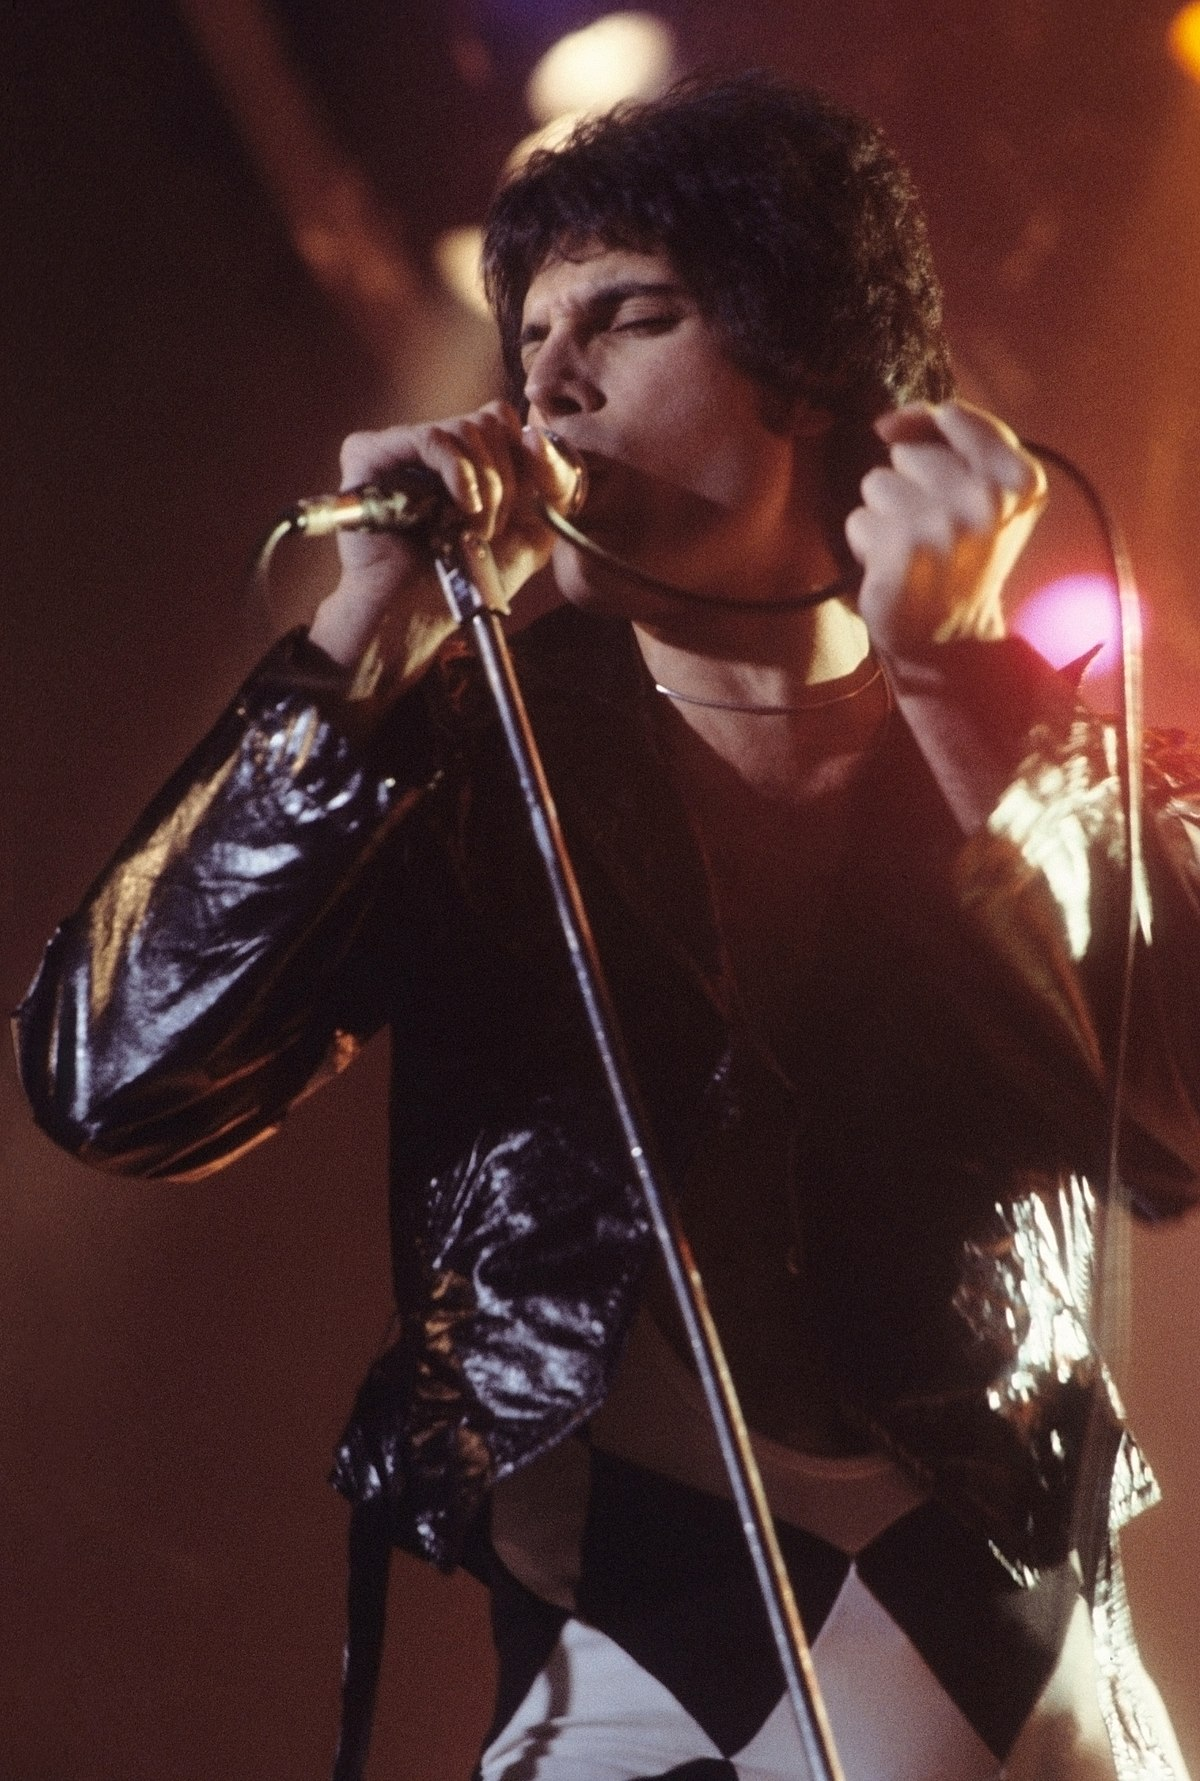
\includegraphics[height=\textwidth]{Freddie.jpg}
      \vspace{-1.0mm}
      \caption{フレディ}
      \label{freddieimg}
  \end{subfigure}
  \begin{subfigure}[b]{0.15\textwidth}
      \centering
      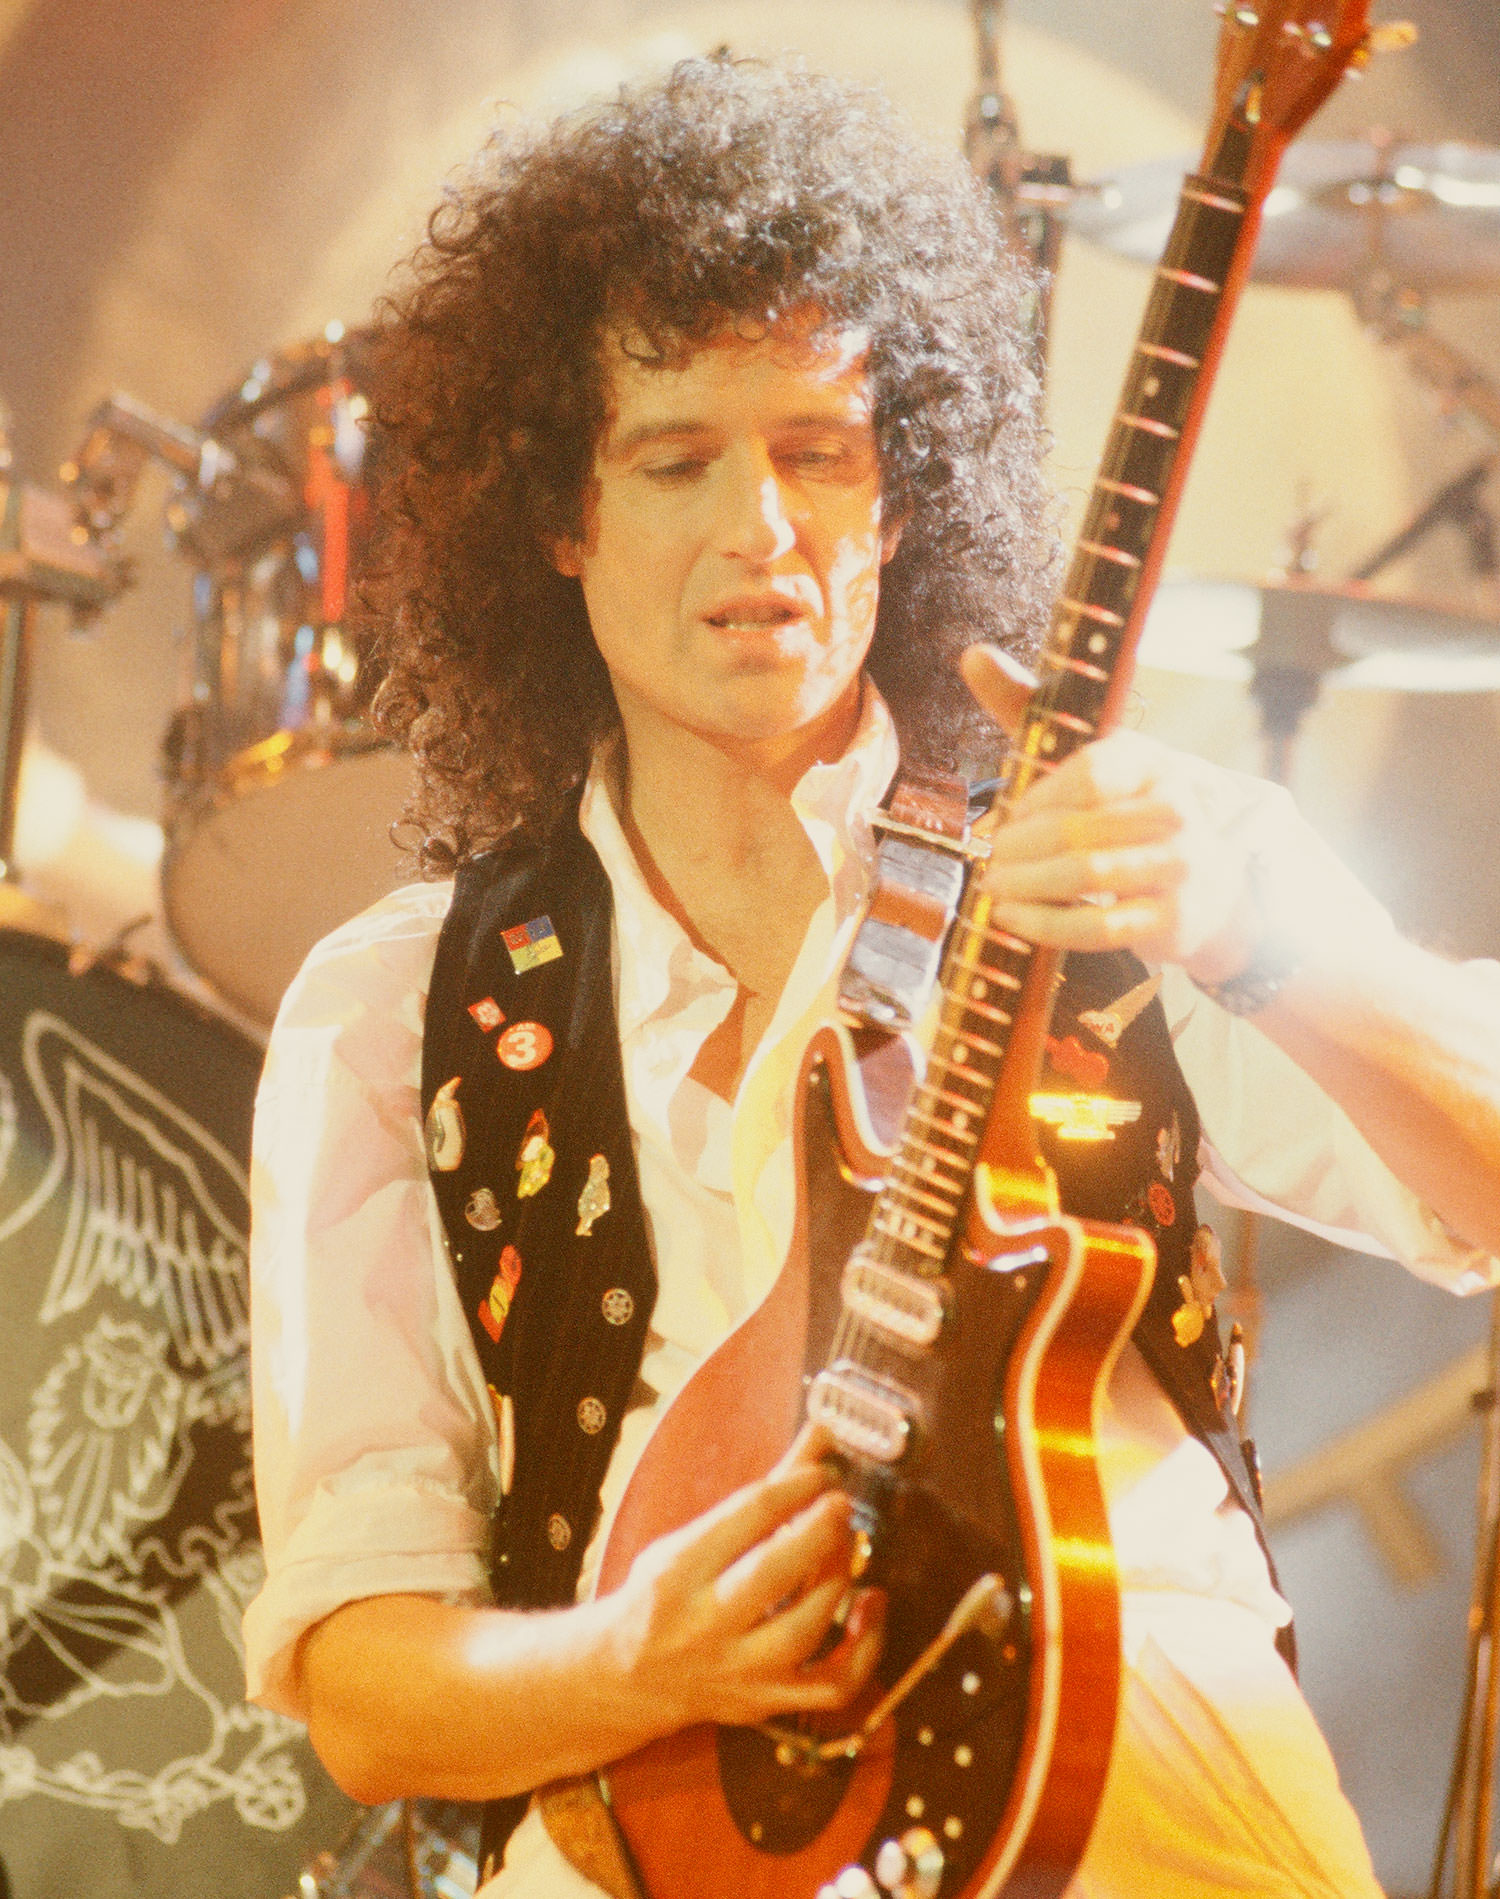
\includegraphics[height=\textwidth]{Brian.jpg}
      \vspace{-1.0mm}
      \caption{ブライアン}
      \label{brianimg}
  \end{subfigure}
  \\
  \begin{subfigure}[b]{0.15\textwidth}
    \centering
    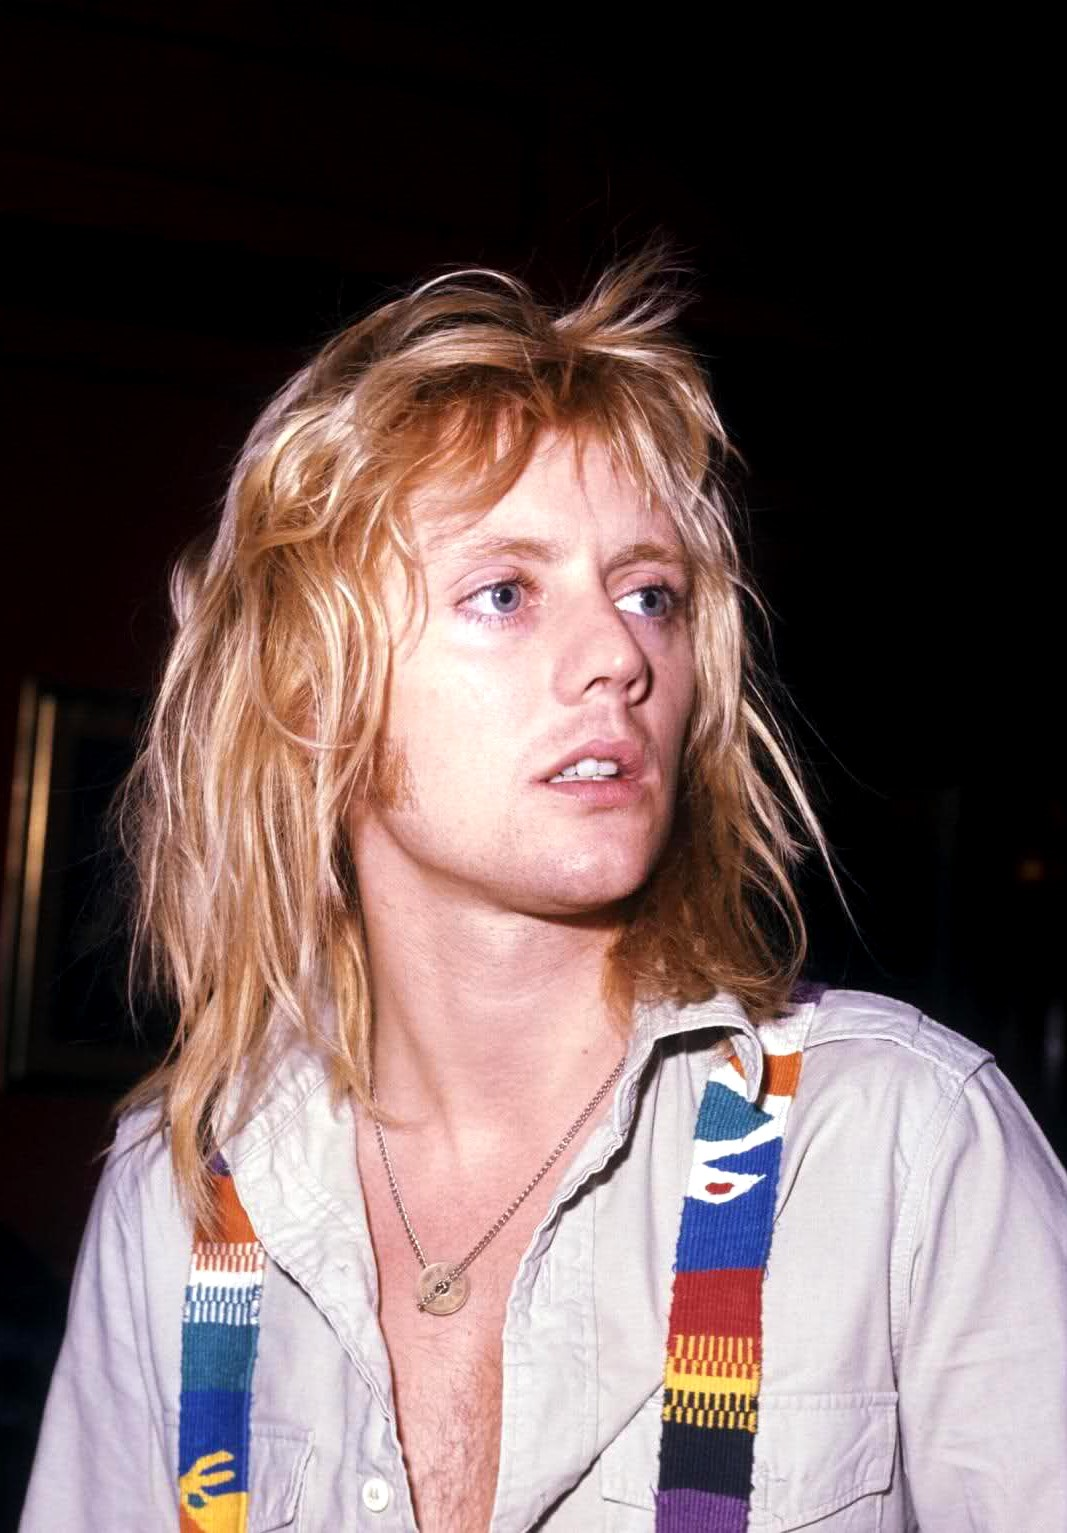
\includegraphics[height=\textwidth]{Roger.jpg}
    \vspace{-1.0mm}
    \caption{ロジャー}
    \label{rogerimg}
  \end{subfigure}
  \begin{subfigure}[b]{0.15\textwidth}
    \centering
    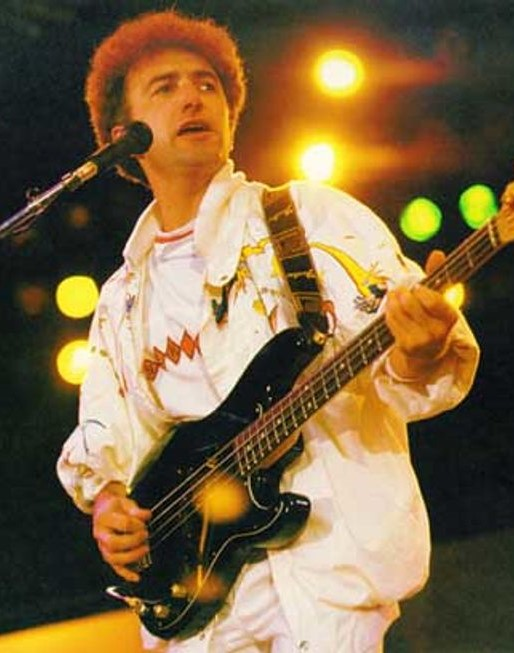
\includegraphics[height=\textwidth]{John.jpg}
    \vspace{-1.0mm}
    \caption{ジョン}
    \label{johnimg}
  \end{subfigure}
      \vspace{-3.0mm}
      \caption{クイーンのメンバー}
     \label{jpnimg}
\end{figure}

\section{クイーンの誕生}

クイーンの結成メンバーは,1960年代後半に西ロンドンで出会った.ギタリストのブライアンメイは翌年,ボーカルのティムスタッフェルと共に1984という名前のグループを結成していた.\cite{Blake}~ ブライアンは1968年初頭,インペリアルカレッジで物理学と赤外線天文学の学位取得に専念するためにグループを脱退し,スタッフェル,キーボーディストのクリススミスと「Smile」というグループを結成した.\cite{Blake}

ラインアップを完成するためにブライアンが大学の掲示板にドラマーを求める広告を出し,若い歯科学生だったロジャーテイラーがオーディションを受けてこの仕事にありつけた.\cite{Hodkinson}

1970年,スタッフェルはソウルとR\&Bへの興味がグループのハードロックサウンドと衝突すると感じ,成功しないことに嫌気がさしてスマイルを脱退した.\cite{Blake} 残ったメンバーはフレディブルサラをリードボーカルとして受け入れた.そして,フレディは,グループ名を「クイーン」に変更することを提案した.

1971年2月,ジョンディーコンがクイーンに加入した.経験豊富なベーシストであることに加え,彼の静かな物腰はバンドを引き立て,エレクトロニクスに長けていた.\cite{Blake}

\begin{figure}[htb]
  \begin{center}
      
\includegraphics[scale=0.3]{Queen.jpg}
      \caption{クイーンのロゴ}
      \vspace{-15pt}
      \label{Queen_Image}
  \end{center}
\end{figure}

\section{アルバム}

クイーンは,ハーモニー,複雑なアレンジ,多様なジャンルの音楽など,ユニークな音を持っています.そのため,彼らのアルバムのほとんどは世界中で売れた.

\vspace{-5pt}

\begin{table}[h]
  \caption{アルバムのチャート順位}
  \vspace{-20pt}
  \label{Album_Table}
  \begin{center}
    \begin{tabular}{|c|c|c|c|}
      \hline
                                 &               & \multicolumn{2}{|c|}{順位}\\[0.50ex] \cline{3-4}
      \raisebox{1.5ex}{アルバム名}& \raisebox{1.5ex}{アルバム発売}   
      & UK & JPN\\ [0.50ex] \hline
      Queen                      & 1973年  & 24 & 52\\ \hline
      Queen II                   & 1974年  & 5  & 26\\ \hline
      A Night at the Opera       & 1975年  & 1  & 1 \\ \hline
      A Day at the Races         & 1976年  & 1  & 1 \\ \hline
      News of the World          & 1977年  & 4  & 3 \\ \hline
      Jazz                       & 1978年  & 2  & 5 \\ \hline
    \end{tabular}
  \end{center}
\end{table}

\vspace{-25pt}

\section{名曲}
クイーンの名曲をいくつか紹介する.
\begin{description}
  \item[ボヘミアンラプソディー] :人を殺し,悪魔に魂を売ってしまった若者の物語である.
  \item[アンダープレッシャー] :フレディとボウイのデュエットソング.
  \item[キラークイーン] :高級風俗嬢を描いたこのグラム時代の名作を見事に表現した.
  \item[ラジオガガ]: 商業化され,同じ曲を繰り返し流すようになったラジオ局を批判した.
  \item[ドントストップミーナウ] :フレディが止められない気持ちを表している.
  \item[サムバディトゥラブ]: 傷つき,落ち込んだ男が,愛する人を見つけることで,この精神状態から抜け出してくれるよう神に懇願する物語である.
  \item[ウィーアーザチャンピオンズ] :逆境を乗り越え,試練を乗り越え,勝利すること.
\end{description}

\section{名曲:ボヘミアンラプソディーー}
4枚目のアルバム「A Night at the Opera」(1975年)からのリードシングルとしてリリースされた「ボヘミアンラプソディー」.リードボーカルのフレディマーキュリーによって書かれた.

\begin{figure}[htb]
  \begin{center}
      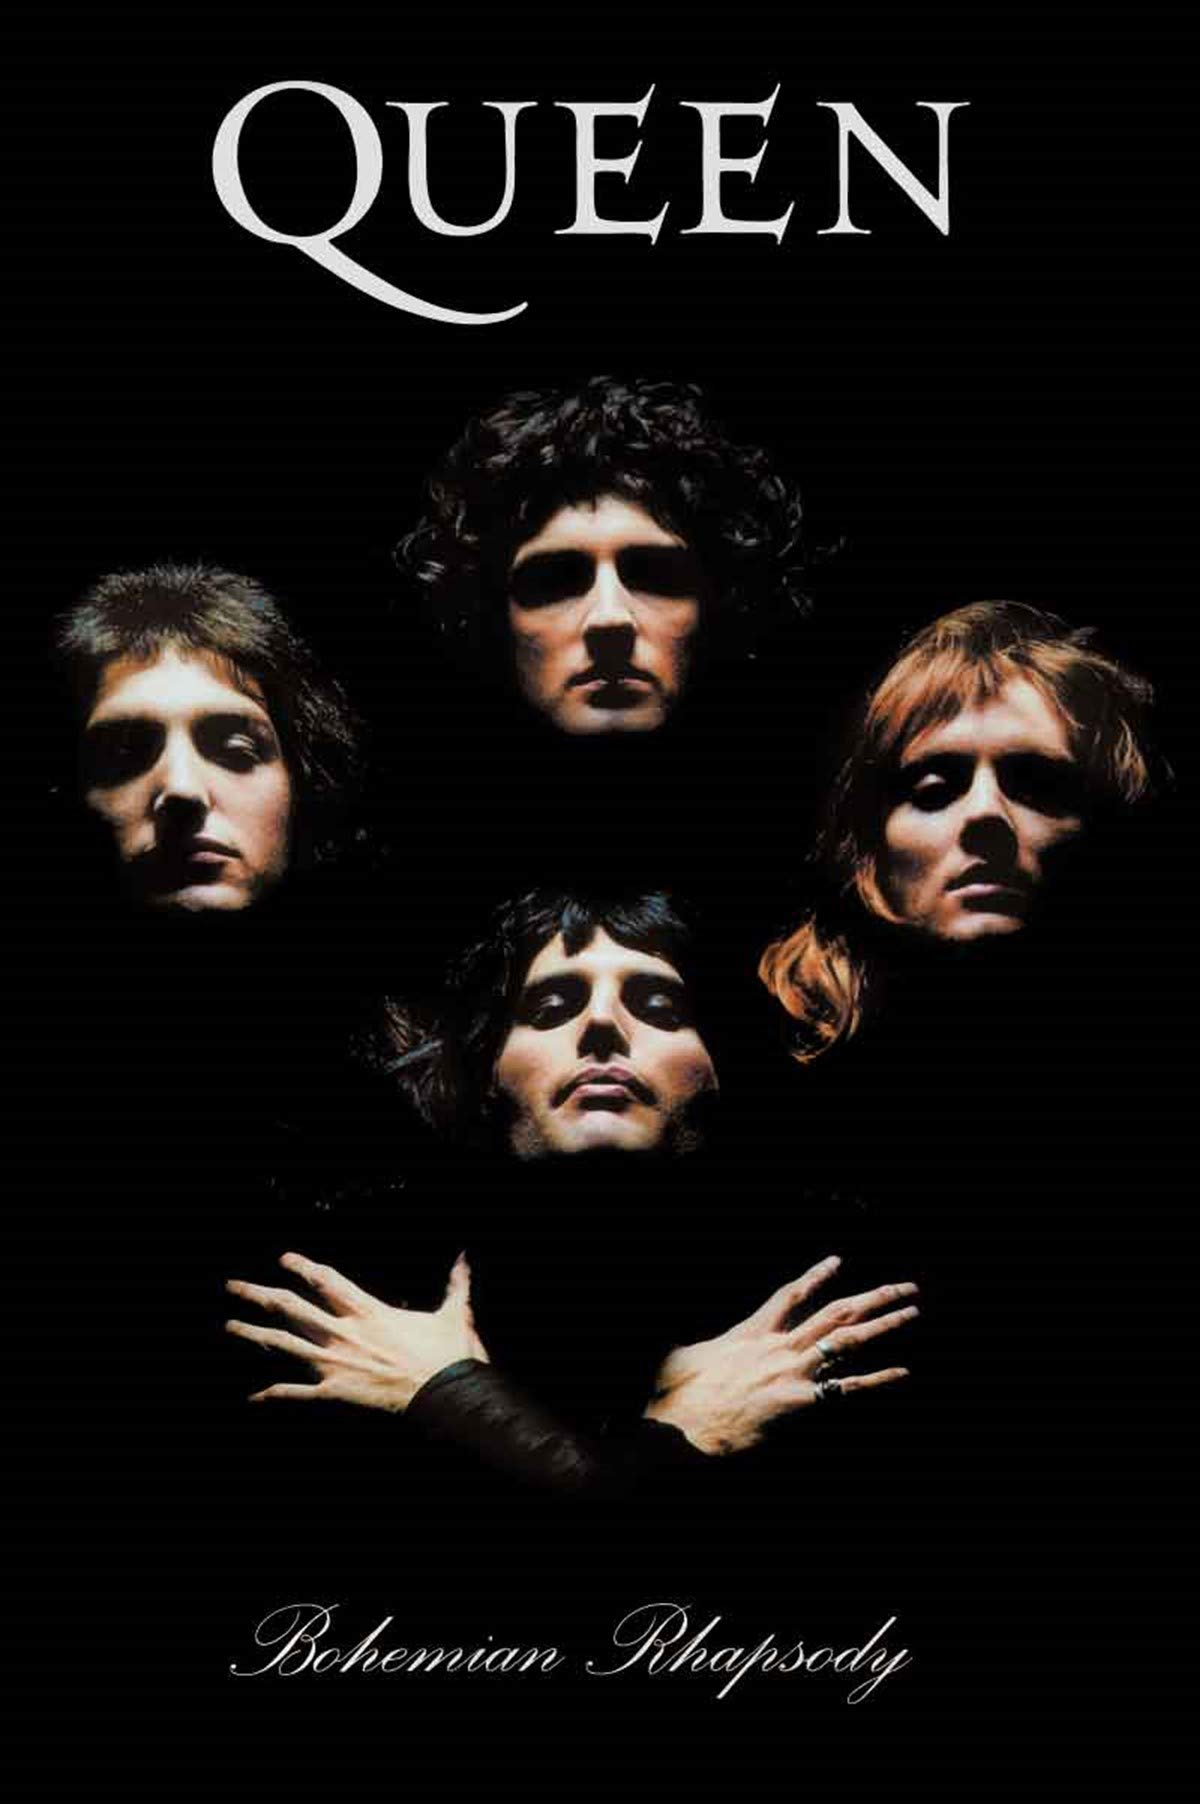
\includegraphics[scale=0.1]{Bohemian.jpg}
      \caption{ボヘミアンラプソディーのポスター}
      \vspace{-15pt}
      \label{Bohemian}
  \end{center}
\end{figure}

「ボヘミアンラプソディー」と呼ばれるのは,「ボヘミアン」の人生を描いているためです.ボヘミアンの本来の意味は「芸術家」ですが,「ラプソディ」はファンタジー(彼の頭の中で再生される可能性があります)またはビジョンです. この曲の中で,フレディマーキュリーは象徴的な方法で自分の人生を予見しています.

クイーンは,「ボヘミアンラプソディー」は,誤って人を殺してしまい,悪魔に魂を売ってしまった若者の話だと述べています.処刑前夜,彼は「ビスミッラー」(アラビア語で「神の名において」)と言って神を呼び,天使の助けを借りてシャイターン(アラビア語で悪魔)から魂を取り戻す.

\section{クイーンに関するドキュメンタリー映画}
名曲「ボヘミアンラプソディー」にちなんで名付けられた映画である.
「ボヘミアンラプソディー」は,イギリスのロックバンド「クイーン」のリードボーカル,フレディマーキュリーの1970年のバンド結成から1985年の本家ウェンブリースタジアムでのライブエイド出演までの人生に焦点を当てた2018年の伝記音楽ドラマ映画である.

\vspace{-15pt}

\subsection{功績}
\subsubsection{2019年アカデミー賞,アメリカ}
\begin{itemize}
  \item 最優秀主演男優賞:ラミマレック
  \item 映画編集部門最優秀賞:ジョンオットマン
  \item 音響編集部門最優秀賞:ジョンウォーハースト,ニナ・ハートストーン
  \item サウンドミキシング部門最優秀賞:ポールマッシー,ティムカヴァギン,ジョンカサリ
\end{itemize}
\vspace{-25pt}
\subsubsection{2019年BAFTA賞}
\begin{itemize}
  \item 最優秀主演男優賞:ラミマレック
  \item 撮影賞:ニュートントーマスシゲル
\end{itemize}
\vspace{-25pt}
\subsubsection{2019年ゴールデングローブ賞,アメリカ}
\begin{itemize}
  \item 映画作品賞(ドラマ部門):ボヘミアンラプソディー
  \item 最優秀男優賞(ドラマ部門):ラミマレック
\end{itemize}
\vspace{-20pt}
\subsection{歴史的正確性}
この映画は,バンドのキャリアやマーキュリーの私生活における出来事を架空または誇張していると批判されている.\cite{Baillie}~ この映画は現実の出来事と比較すると79.9\%正確であると推測し,「大量に圧縮(および編集)した時間軸で表現したかなり真実に近い説明」であるとした.\cite{Site}

\section{音の強さ}

音響インテンシティは,以下の式から求めることがでる:

\begin{equation}
  \label{eq1}
  I = 
  \frac{
    \Delta p^2
  }{
    2\rho V_w
  }
\end{equation}

\vspace{15pt}
圧力変化$\Delta p$, 物質の密度を$\rho$,速さを$V_w$.

ちなみに,ロックコンサートは空間に関係なく,非常に大きな音を出すことができます.平均して,ロックコンサートのデシベルレベルは$90 ~ 120 dB$です.

\section{まとめ}

1991年11月22日にフレディを亡くした後も,クイーンは皆の心の中に特別な位置を占めている.
2002年,クイーンの「ボヘミアンラプソディー」は,ギネスワールドレコーズブリティッシュヒットシングルブックが行った投票で,「イギリスで最も好きなヒット曲」に選ばれている.

2004年末,ブライアンとロジャーは,2005年にポールロジャース(フリーとバッドカンパニーの創設者で元リードボーカル)と再結成してツアーに復帰することを発表した.ブライアンメイのウェブサイトには,ロジャースはフレディの代わりではなく「クイーン+ポールロジャース」としてクイーンと共に「フィーチャー」されるとも書かれていた.引退していたディーコンは参加しなかった.クイーンとポールロジャースは2009年5月12日に反目することなく正式に離婚した.

2009年,アメリカンアイドルの撮影現場で出会ったアダムランバートを,クイーンは選んだ.彼らは「Queen + Adam Lambert」となり,今日までパフォーマンスを続けています.

\begin{figure}[htb]
  \begin{center}
      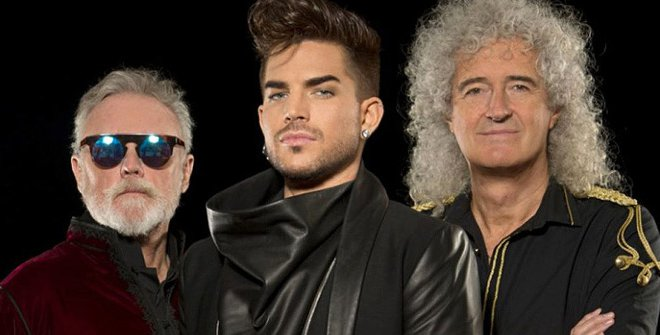
\includegraphics[scale=0.3]{queen_adam_lambert.jpg}
      \caption{Queen + Adam Lambert}
      \vspace{-15pt}
      \label{QueenAdam}
  \end{center}
\end{figure}

\vspace{-15pt}

\begin{thebibliography}{99}
  \bibitem{Blake}
  Blake, Mark (2016). Freddie Mercury: A Kind of Magic. Omnibus Press.
  \bibitem{Hodkinson}
  Hodkinson, Mark (2004). Queen: The Early Years. London: Music Sales Limited.
  \bibitem{Baillie}
  https://www.noted.co.nz/culture/movies/bohemian-rhapsody-kiwi-anthony-mccarten-wrote-queen-movie/(参照2023-05-16)
  \bibitem{Site}
  https://www.informationisbeautiful.net/visualizations/ based-on-a-true-true-story/(参照2023-05-16)

\end{thebibliography}
\end{document}